\begin{figure*}[t!]
    \centering
    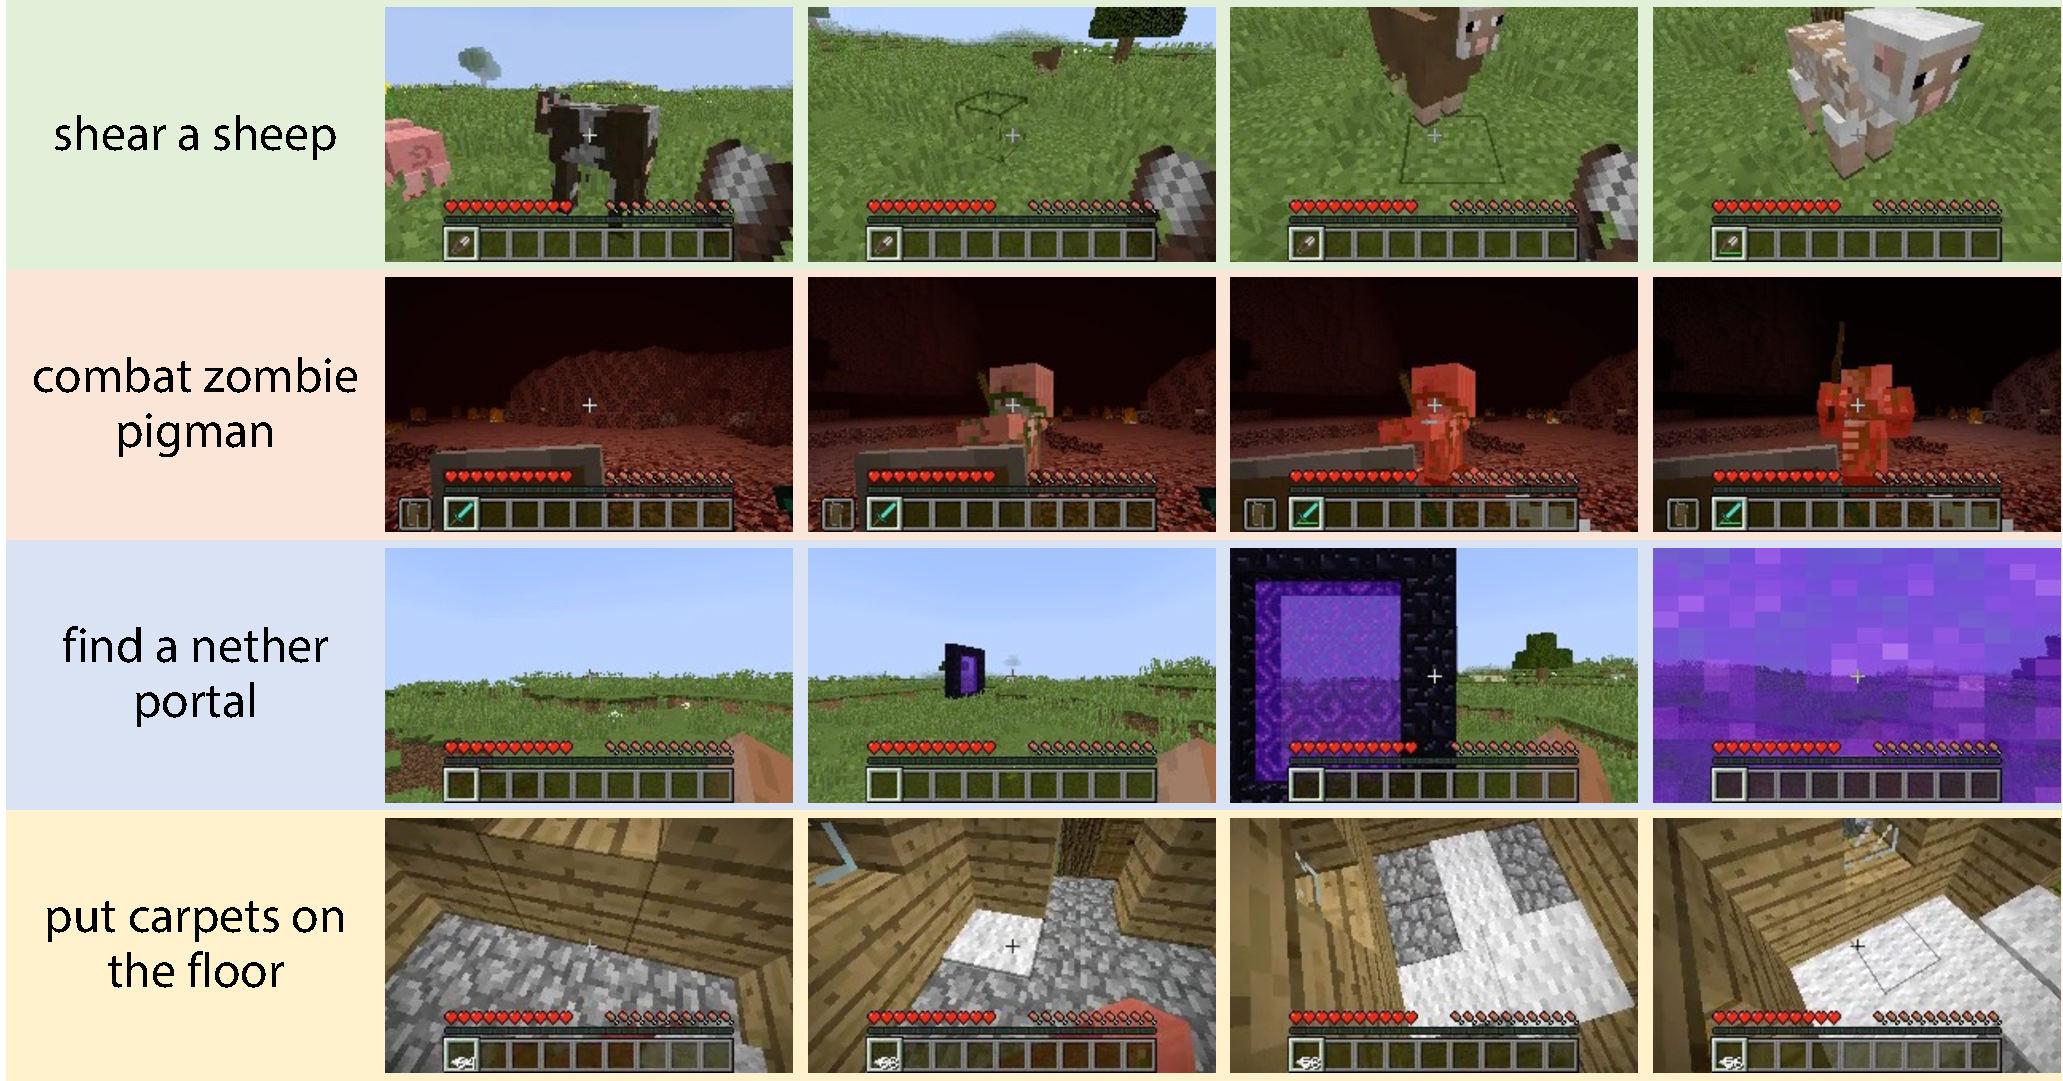
\includegraphics[width=\linewidth]{figs/behavior_visualization-fig.pdf}
    \caption{Visualization of our agent's learned behaviors on four selected tasks. Leftmost texts are the task prompts used in training. Best viewed on a color display.}
    \label{fig:behavior_visualization}
\end{figure*}
\section{\minedojo Simulator \& Benchmark Suite}
\label{sec:benchmark}
\minedojo offers a set of simulator APIs help researchers develop generally capable, open-ended agents in Minecraft. 
It builds upon the open-source MineRL codebase \cite{guss2019minerl} and makes the following upgrades: 
1) We provide \textbf{unified observation and action spaces} across all tasks, facilitating the development of multi-task and continually learning agents that can constantly adapt to new scenarios and novel tasks. This deviates from the MineRL Challenge design that tailors observation and action spaces to individual tasks;
2) Our simulation unlocks all three types of worlds in Minecraft, including the \textit{Overworld}, the \textit{Nether}, and the \textit{End}, which \textbf{substantially expands the possible task space}, while MineRL only supports the Overworld natively; and 3) We provide convenient APIs to configure initial conditions and world settings to standardize our tasks. 

With this \minedojo simulator, we define thousands of benchmarking tasks, which are divided into two categories: 1) \textit{Programmatic tasks} that can be automatically assessed based on the ground-truth simulator states; 
and 2) \textit{Creative tasks} that do not have well-defined or easily-automated success criteria, which motivates our novel evaluation protocol using a learned model (Sec. \ref{sec:method}). 
To scale up the number of Creative tasks, we mine ideas from YouTube tutorials and use OpenAI's GPT-3~\cite{brown2020gpt3} service to generate substantially more task definitions. 
Compared to Creative tasks, Programmatic tasks are simpler to get started, but tend to have restricted scope, limited language variations, and less open-endedness in general.

\subsection{Task Suite I: Programmatic Tasks}
\label{sec:benchmark-programmatic}
We formalize each programmatic task as a 5-tuple: $T = (G, \mathcal{G}, \mathcal{I}, f_\mathcal{S}, f_\mathcal{R})$. 
$G$ is an English description of the task goal, such as ``\textit{find material and craft a gold pickaxe}''. 
$\mathcal{G}$ is a natural language guidance that provides helpful hints, recipes, or advice to the agent.
We leverage OpenAI's \texttt{GPT-3-davinci} API to automatically generate detailed guidance for a subset of the tasks.
For the example goal ``\textit{bring a pig into Nether}'', GPT-3 returns: \texttt{1) Find a pig in the overworld;
2) Right-click on the pig with a lead;
3) Right-click on the Nether Portal with the lead and pig selected;
4) The pig will be pulled through the portal!}
$\mathcal{I}$ is the initial conditions of the agent and the world, such as the initial inventory, spawn terrain, and weather.
$f_\mathcal{S}$: $s_t \rightarrow \{0, 1\}$ is the success criterion, a deterministic function that maps the current world state $s_t$ to a Boolean success label. 
$f_\mathcal{R}$: $s_t \rightarrow \mathbb{R}$ is an optional dense reward function. We only provide $f_\mathcal{R}$ for a small subset of the tasks in \minedojo due to the high costs of meticulously crafting dense rewards. \Rebuttal{For our current agent implementation (\mbox{Sec. \ref{sec:method-mineclip-pretraining}}), we do not use detailed guidance. Inspired by concurrent works SayCan~\mbox{\cite{ahn2022saycan}} and Socratic Models~\mbox{\cite{zeng2022socratic}}, one potential idea is to feed each step in the guidance to our learned reward model sequentially so that it becomes a stagewise reward function for a complex multi-stage task.}

\minedojo provides 4 categories of programmatic tasks with 1,581 template-generated natural language goals to evaluate the agent's different capabilities systematically and comprehensively: 

\begin{enumerate}[leftmargin=3em]
    \item \textbf{Survival}: surviving for a designated number of days.
    \item \textbf{Harvest}: finding, obtaining, cultivating, or manufacturing hundreds of materials and objects.
    \item \textbf{Tech Tree}: crafting and using a hierarchy of tools.
    \item \textbf{Combat}: fighting various monsters and creatures that require fast reflex and martial skills.
\end{enumerate}

Each task template has a number of variations based on the terrain, initial inventory, quantity, etc., which form a flexible spectrum of difficulty. In comparison, the NeurIPS MineRL Diamond challenge \cite{guss2019minerl} is a subset of our programmatic task suite, defined by the task goal ``\textit{obtain 1 diamond}" in \minedojo.  

\subsection{Task Suite II: Creative Tasks}
\label{sec:benchmark-creative}

We define each creative task as a 3-tuple, $T = (G, \mathcal{G}, \mathcal{I})$, which differs from programmatic tasks due to the lack of straightforward success criteria. 
Inspired by model-based metrics like the Inception score~\cite{DBLP:conf/nips/SalimansGZCRCC16} and FID score~\cite{DBLP:conf/nips/HeuselRUNH17} for image generation, we design a novel task evaluation metric based on a pre-trained contrastive video-language model (Sec. \ref{sec:method-mineclip-pretraining}). In the experiments, we find that the learned metric exhibits a high level of agreement with human evaluations (see Table \ref{table:eval-metric-quality}).  

We brainstorm and author 216 Creative tasks, such as ``\textit{build a haunted house with zombie inside}'' and ``\textit{race by riding a pig}''. Nonetheless, such a manual approach is not scalable. Therefore, we develop two systematic approaches to extend the total number of task definitions to 1,560. This makes our Creative tasks \textit{3 orders of magnitude} larger than Minecraft BASALT challenge \cite{shah2021basalt}, which has 4 Creative tasks.

\para{Approach 1. Task Mining from YouTube Tutorial Videos.} We identify our YouTube dataset as a rich source of tasks, as many human players demonstrate and narrate creative missions in the tutorial playlists. To collect high-quality tasks and accompanying videos, we design a 3-stage pipeline that makes it easy to find and annotate interesting tasks (see Sec.~\ref{supp:sec:creative_tasks} for details).
Through this pipeline, we extract 1,042 task ideas from the common wisdom of a huge number of veteran Minecraft gamers, such as ``\textit{make an automated mining machine}'' and ``\textit{grow cactus up to the sky}''. 

\para{Approach 2. Task Creation by GPT-3.} We leverage GPT-3's few-shot capability to generate new task ideas by seeding it with the tasks we manually author or mine from YouTube. The prompt template is: \texttt{Here are some example creative tasks in Minecraft: \{a few examples\}. Let's brainstorm more detailed while reasonable creative tasks in Minecraft}.\\
GPT-3 contributes 302 creative tasks after de-duplication, and demonstrates a surprisingly proficient understanding of Minecraft terminology.

\subsection{Collection of Starter Tasks}

\Rebuttal{We curate a set of 64 core tasks for future researchers to get started more easily. If their agent works well on these tasks, they can more confidently scale to the full benchmark. }

\begin{itemize}[leftmargin=2em,labelsep=0.7em]
    \item \textbf{32 programmatic tasks}: 16 ``standard'' and 16 ``difficult'', spanning all 4 categories (survival, harvesting, combat, and tech tree). We rely on our Minecraft knowledge to decide the difficulty level. ``Standard'' tasks require fewer steps and lower resource dependencies to complete. 
    \item \textbf{32 creative tasks}: 16 ``standard'' and 16 ``difficult''. Similarly, tasks labeled with ``standard'' are typically short-horizon tasks. 
\end{itemize}

\Rebuttal{We recommend that researchers run 100 evaluation episodes for each task and report the percentage success rate. The programmatic tasks have ground-truth success, while the creative tasks need our novel evaluation protocol (Sec.~\mbox{\ref{sec:experiments}}). }
